\documentclass{article}
\usepackage[utf8]{inputenc}
\usepackage{amsmath,amsfonts,amssymb}
\usepackage[margin=1in]{geometry}
\usepackage[parfill]{parskip}
\usepackage{authblk}
\usepackage{graphicx}
\usepackage{xcolor}

% for nice url formatting, including auto linebreaks
\usepackage{xurl}

% makes nice looking tables
\usepackage{tabularx}

% get periods in figure captions instead of colons
\usepackage[labelsep=period]{caption}

\title{Improved criteria for evaluation of proteomics imputation methods and recommendations for the future}

\newcommand{\fixme}[1]{{\color{red}{#1}}}

\author[1]{Lincoln Harris}
\author[2]{William E. Fondrie}
\author[3]{Seewong Oh}
\author[1,3]{William S. Noble}

\affil[1]{Department of Genome Sciences, University of Washington}
\affil[2]{Talus Biosciences}
\affil[3]{Paul G.\ Allen School of Computer Science and Engineering,
  University of Washington}

\date{January 2022}

\begin{document}

\maketitle

\begin{abstract}
\noindent
\small
Mass spectrometry-based quantitative proteomics experiments currently suffer from excess missingness. Missingness hinders reproducibility, reduces statistical power and makes it difficult to compare across samples or experiments. While a number of methods exist for imputing missing values in proteomics data, in practice, the most commonly used methods are among the worst performing. Here we evaluate the performance of commonly used imputation methods using a set of practical criteria including differential expression analysis, the number of quantitative peptides and the lower limit of quantitation of peptides in a proteomics experiment. We evaluate performance on a variety of proteomics experiments including isobaric labeled, label free, data independent acquisition and data dependent acqusition. We also argue that existing methods do not properly account for the distribution of peptide quantifications. 

\end{abstract}

\section{Introduction}
The quantitative accuracy and sensitivity of mass spectrometry-based proteomics experiments has increased dramatically in the past decade. In spite of this, quantitative mass spectrometry is still limited by excessive ``missingness'', which refers to peptides that are present in the sample matrix but are not detected by the instrument. Missingness can be attributed to a number of technical factors including poor sample ionization, electrospray instability \fixme{[what does this mean?]}, the lower limit of quantification of the instrument and the inability to confidently assign peptides to all observed spectra \cite{Bramer:review, Webb-Robertson:review}. Missingness decreases the statistical power of proteomics experiments, hinders reproducibility and makes it difficult to compare across batches or experiments \cite{Bramer:review, Webb-Robertson:review}. 

While low abundance peptides are more likely to be missing, missingness can effect peptides across the entire range of intensities \cite{lazar}. Thus, technical solutions to the missingness problem will benefit virtually all quantitative proteomics studies. 

Imputation is one analytical solution to the missingness problem. Imputation entails using statistical or machine learning procedures to estimate missing values in quantitative proteomics experiments. While a large number of imputation methods exist for quantitative proteomics data (for reference, see \cite{Bramer:review, Webb-Robertson:review}), in practice it is not always clear which method is ``best'' for a given dataset. A number of studies offer guidelines and recommendations for selecting an imputation method \cite{Jin, DIMA, lazar, valikangas, dabke}. The majority of these studies evaluate imputation methods with metrics commonly used by the machine learning community, for example, by computing the mean squared error (MSE) between imputed and ground truth peptide quantitations. Here we argue that such “traditional” evaluation criteria are not very relevant to most proteomics researchers, and offer alternative evaluation criteria specifically tailored to the questions proteomics researchers commonly seek to answer. Examples of commonly used imputation methods are given in Table \ref{tab:method-descrip}. 

We also investigate the imputation methods currently used within the community and demonstrate that while a large number of methods exist, in practice, only a small handful are actually used by proteomics researchers. Figure \ref{fig:citation-counts} demonstrates that by far the most commonly used method is the Perseus \cite{Perseus} strategy of randomly sampling from a Gaussian distribution centered about the lowest observed peptide abundance value. In spite of its popularity, this method has been shown to work poorly \cite{Bramer:review, Webb-Robertson:review}. Single-value replacement strategies such as the Perseus method do not properly account for the distribution of missing values in quantitative proteomics experiments. We speculate that the reason for this method's popularity is the fact that it is integrated into the popular Perseus suite of mass spectrometry data processing tools \cite{Perseus}. This suggests the need for more accurate imputation tools that are as easy to use as Perseus, and can be easily integrated into existing data processing pipelines. 

Interesting that we don't find a single PCA-based imputation method in this literature search. 

We choose to focus on imputing at the peptide, rather than protein, level as recent studies have suggested that this is the best practice \cite{humpty-dumpty}.

We also demonstrate that peptide quantifications are neither Gaussian nor Poisson distributed. This is relevant because many existing imputation methods either implicitly or explicitly assume a Gaussian distribution of quantifications. To our knowledge, no existing method models peptide quantifications with the proper distributional assumption. This suggests the need for improved imputation methods that either model quantifications with the proper distributional assumption or employ some form of variance stabilization prior to imputation. We demonstrate that the commonly used log transformation does not stabilize the variance of peptide quantifications. 

We benchmark performance of some of the most commonly used imputation methods including Gaussian random sampling, low value, k-nearest neighbors and \textit{missForest} \cite{knn-impute, missForest}. We also include a non-negative matrix factorization (NMF)-based imputation method. NMF has recently been proposed for proteomics data; thus we choose to include this new and promising method \cite{ms-impute, nmf-metabolomics}. 

Performance is evaluated using traditional criteria such as MSE, in addition to several proteomics specific criteria including the ability of an imputation method to: (i) reconstruct differentially expressed peptides, (ii) increase the number of “quantitative” peptides in a proteomics experiment, and (iii) improve the lower limit of quantification for peptides in a mass spectrometry experiment. We benchmark various imputation methods on a variety of datasets including a dilution series, data-dependent acquisition (DDA), data-independent acquisition (DIA), label-free and isobaric labeled experiments. We find that random forest-based imputation \cite{missForest} reliably works the best across a variety of quantitative proteomics experiments, but call for the development of imputation methods that properly take into account the distribution of peptide quantifications, employ variance stabilization and are flexible enough to handle data from many different types of proteomics experiments. We also recommend that the community move away from “machine learning” style evaluation of imputation methods and use instead the proteomics specific criteria we describe here. 

\begin{table}
  \small
  \centering
  \begin{tabular}{lp{3.5in}r}
  %\begin{tabular}{p{1.5in}p{3.5in}p{1in}}
    \hline
    Method & Description & Examples \\
    \hline
    Zero replacement & Replace missing values with zeros & \\
    Mean replacement & Replace missing values with the mean peptide intensity for a peptide or run & \\
    Low value replacement & Replace missing values with the lowest observed abundance in any sample or run & \\
    \textit{missForest} & Nonparametric method to impute missing values
using a random forest trained on the observed parts of the data set,
repeated iteratively until convergence & \textit{missForest} \cite{missForest} \\
    kNN & Weighted average intensity of $k$ most similar peptides & \textit{VIM}, \textit{impute.knn} \cite{VIM, knn-impute} \\
    Random sample & Randomly sample from a distribution centered around the lowest observed abundance & Perseus \cite{Perseus} \\
    PCA & Run principal component analysis, impute missing values with the regularized reconstruction formulas and repeat until convergence & \textit{pcaMethods}, \textit{missMDA} \cite{pcaMethods, missMDA} \\
    Regression & Linear regression is used to estimate missing values & \textit{lm, glm} \\
    \hline
  \end{tabular}
  \caption{{\bf Existing MS/MS imputation methods.} Descriptions of general categories of imputation strategies for quantitative proteomics data and examples of methods that implement each general strategy. Italics indicate R packages. 
    \label{tab:method-descrip}}
\end{table}

\begin{figure}
\centering
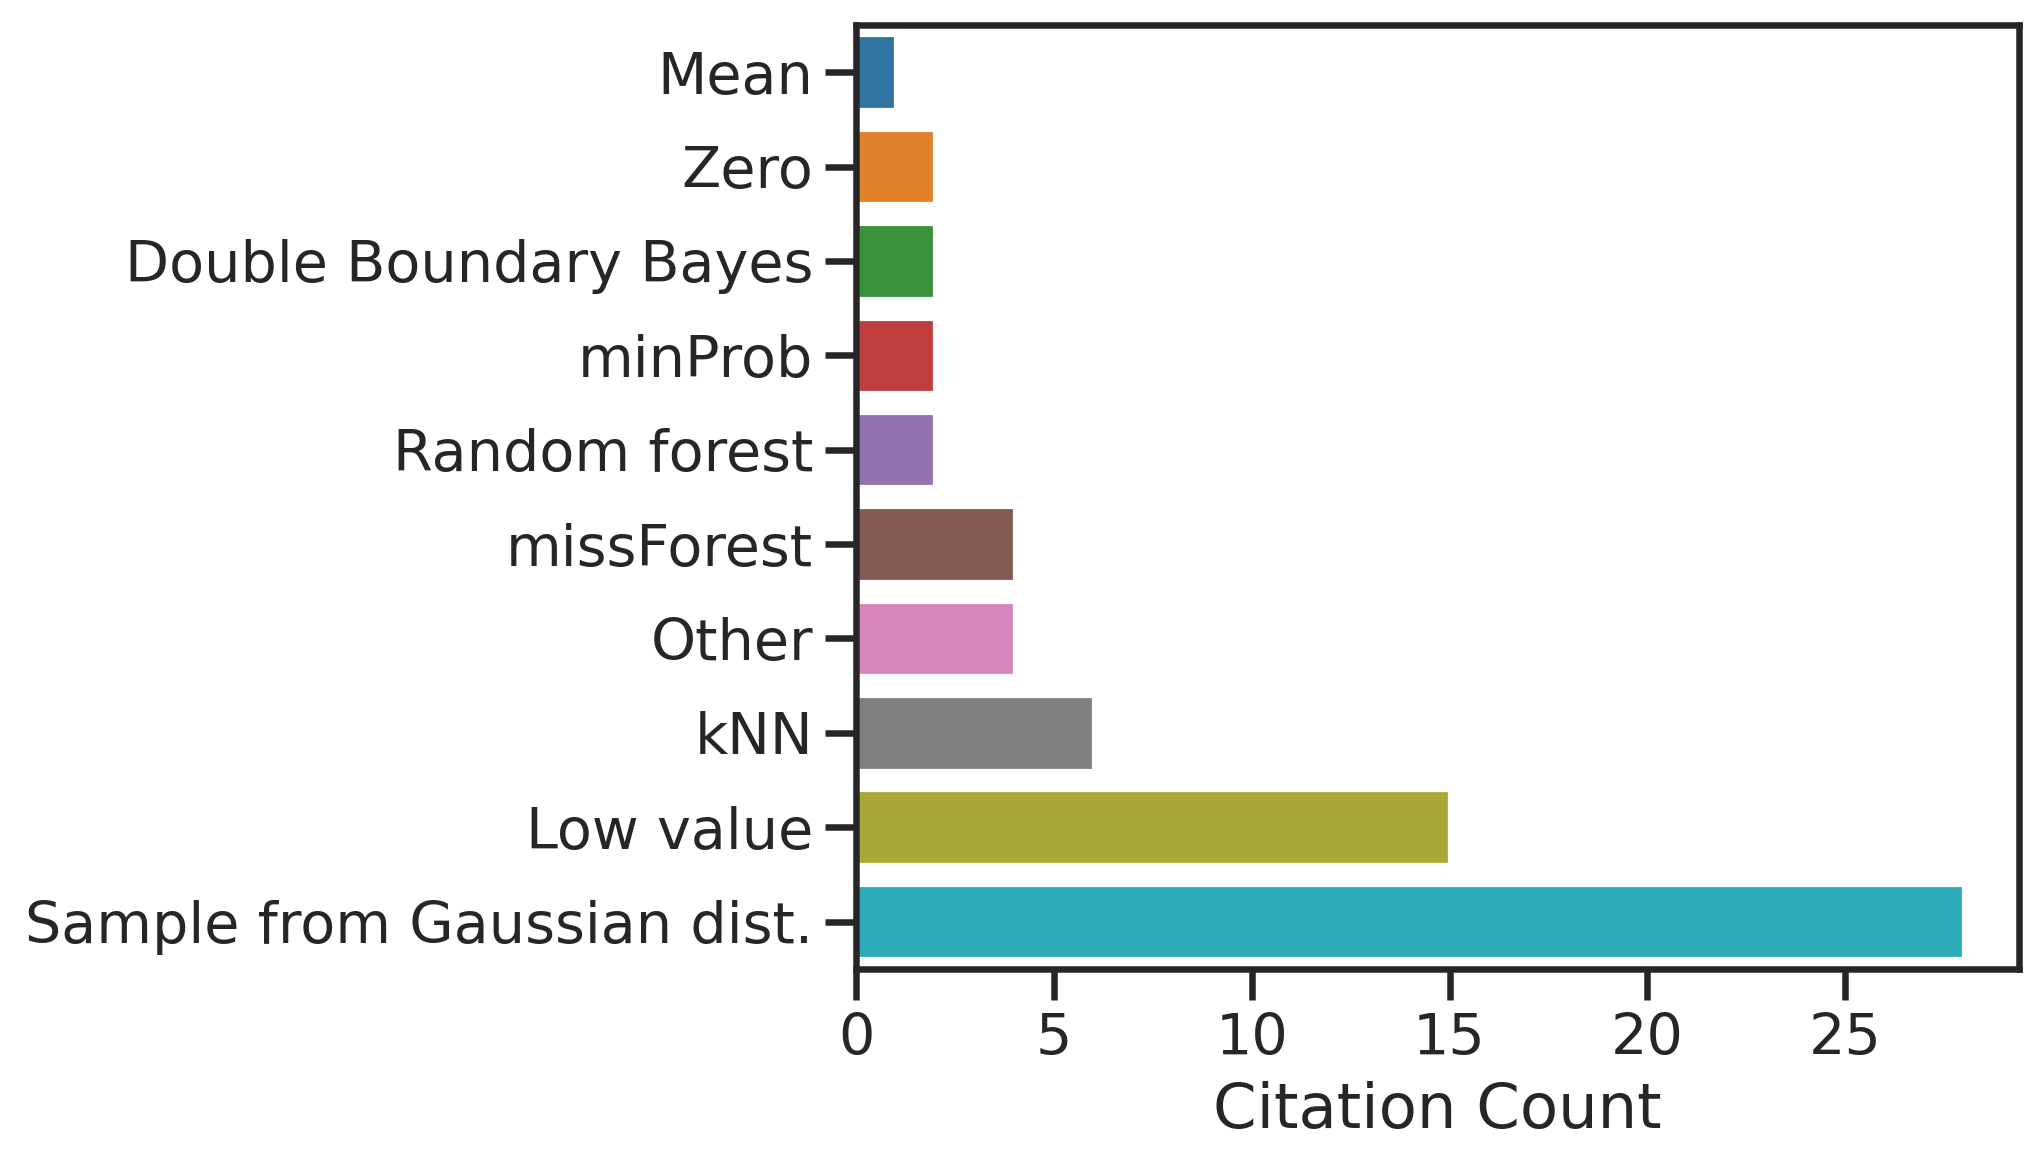
\includegraphics[width=0.7\textwidth]{figures/imp-lit-seq-results-update.png}
\caption{{\bf Citation counts for the most commonly used MS/MS imputation methods.} Literature survey of \textit{Journal of Proteome Research} articles, January 2019 -- January 2023. Methods labeled “other” appear in just a single publication, and refer to ``imp4p'', ``QRLIC'', ``Euclidean distances'' and ``random draw from the entire peptide abundance range''.}
\label{fig:citation-counts}
\end{figure}

\section{Methods}
\textit{Journal of Proteome Research} articles published between January 1\textsuperscript{st}, 2019 and January 31\textsuperscript{st}, 2023 were searched for the following terms: ``impute'', ``imputed'' and ``imputation''. The results are reported in Figure \ref{fig:citation-counts}. This figure only considers research articles, that is, methodological and benchmarking studies are not included in the citation counts. The full results of this literature search, including the names and DOIs of the identified studies, are included as \fixme{Supplemental Table 1}. 

Characteristics of the 11 public quantitative proteomics datasets analysed in this study are provided by Table \ref{tab:data-description}. Nine of the 11 datasets were accessed via the Proteomics Identification Database (\url{https://www.ebi.ac.uk/pride/}) (PRIDE) \cite{PRIDE}, and are indicated with their ProteomeXchange (PXD) labels \cite{ProteomeXchange}. The remaining two datasets were obtained from the National Cancer Institute's Clinical Proteomic Tumor Analysis Consortium (CPTAC) data portal (\url{https://proteomic.datacommons.cancer.gov/pdc/}). The CPTAC dataset identifiers are provided. Peptide-spectrum match files were processed and converted to matrix format with custom scripts (available at \fixme{\url{https://github.com/Noble-Lab/xxx}}). A complete list of the files obtained from each dataset is provided in \fixme{Supplemental Table 2}. 

The peptide quantification matrices from the two CPTAC studies are extremely large (S047: 110k peptides x 226 samples; S051: 291k peptides x 35 samples). To ensure the tractability of our benchmarking study, we downsampled both of these matrices by randomly selecting 40k peptides and 30 runs from each. These downsampled matrices are described in Table \ref{tab:data-description} and were used for analysis. 

For experiments processed with MaxQuant, we gathered peptide quantifications from the \textit{peptides.txt} files. We retained the ``Sequence'' and various ``Intensity'' columns to generate peptide-by-runs intensity matrices. 

For differential expression analysis we obtained data from PXD034525, a DIA study of Alzheimer's disease (AD) \cite{smtg-maccoss}. Clinical samples were obtained and assigned to experimental groups based on a number of genetic, histopathological and behavioral phenotypes. We compared differentially expressed peptides between (i) autosomal dominant AD dementia and (ii) high cognitive function, low AD neuropathologic change. The two experimental groups each had nine samples (each from separate patients) and 32,614 detected peptides. 

Ground truth differentially expressed peptides were determined by performing two-sample t-tests between experimental groups for each detected peptide. P-values were corrected with Benjimani-Hochberg, and any peptide with a corrected p-value $<$ 0.01 was declared ground truth differentially expressed.

Missing values were then simulated into the two peptide quantification matrices with two different procedures: missing completely at random (MCAR) and missing not at random (MNAR). For MCAR, 15\% of the present matrix entries were randomly selected for both the validation and test sets. The remaining matrix entries were used as the training set. 

For MNAR, we took a similar approach to the one described in Lazar et al., 2016 \cite{lazar}. For a given peptide quantifications matrix, we constructed an equally sized thresholds matrix filled with values sampled from a Gaussian distribution centered about the 30\textsuperscript{th} percentile of the peptide quantifications distribution, with standard deviation 0.6. For each matrix element $X_{ij}$, if the corresponding thresholds matrix element $T_{ij} < X_{ij}$, assign $X_{ij}$ to the training set. Else, conduct a single Bernoulli trial with probability of success 0.75. If success, $X_{ij}$ is assigned alternatively to the validation and test sets. Else, $X_{ij}$ is assigned to the training set. 

For both MNAR and MCAR, peptides that were initially missing were excluded from the training sets. Additionally, peptides with fewer than four present values post-partitioning were removed from both train, validation and test sets prior to imputation. The python scripts used to implement these procedures can be found at \fixme{\url{https://github.com/Noble-Lab/xxx}}.

Once missing values had been simulated into the peptide quantifications matrices for the two experimental conditions from PXD034525, a number of procedures were used for imputation. A custom PyTorch model was used for non-negative matrix factorization (NMF) imputation. This model uses stochastic gradient descent to converge on an ideal matrix factorization. Mean squared error (MSE) was used as the loss function. This model is available at \fixme{\url{https://github.com/Noble-Lab/xxx}}. For \textit{k}-nearest neighbors (kNN) impute, we used the \textit{KNNImputer} implementation from \textit{scikit-learn}. Custom code was used for sample min and Gaussian sample impute. \textit{MissForest} impute was also used \cite{missForest}. 

For NMF and kNN we searched across the following hyperparameters to obtain the optimal \textit{n} latent factors and \textit{k} neighbors, respectively: $[1,2,4,8,16,32]$. For \textit{missForest} a full hyperparameter search proved computationally unfeasible, so we selected the default value of 100 for the \textit{n} trees parameter. The validation set was used to select the optimal hyperparameter for NMF and kNN. The rest of the imputation methods do not have tunable hyperparameters, so hyperparameter searching was not performed. 

Following hyperparameter selection, imputation was performed with each method. The validation and test sets were reconstructed with each imputation method. Differentially expressed peptides were determined for the imputed matrices as previously described. Precision Recall curves comparing ground truth to imputed differentially expressed peptides were generated with \textit{scikit-learn}. For the ``no impute'' condition, the differential expression calculation was performed in the same manner, while simply ignoring the missing matrix entries. That is, the differential expression test was performed on training set values only. 

For examining the effects of imputation on the number of quantitative peptides in a proteomics experiment, we obtained data from PXD014815 \cite{matrix-matched-calib}. This is a serial dilution experiment in which yeast peptides were spiked into a background matrix at various known concentrations. A statistical model was then used to fit the relationship between the observed and expected signal and to determine the lower limit of quantification for each detected peptide. The script implementing this statistical model can be found at \url{https://bitbucket.org/lkpino/matrix-matched_calcurves}. We used this model to assess the number of quantitative peptides before and after imputation of the serial dilutions dataset with various methods. MCAR partitioning was performed as described above. Hyperparameter tuning for kNN and NMF was performed as described above. The \textit{UpsetR} package was used to generate Figure \ref{fig:rescue-experiment} \cite{UpsetR}.

We next used the serial dilution experiment from PXD014815 to examine the effects of imputation on the lower limit of quantification (LLOQ) of peptides. We used scripts found at \url{https://bitbucket.org/lkpino/matrix-matched_calcurves} to determine the LLOQ of all detected peptides before and after imputation. One-sided binomial tests were performed to determine whether each imputation method decreases the LLOQ for more peptides than it increases. Binomial p-values were corrected with the Benjimani-Hochberg procedure. 

We next used a traditional machine learning setup to evaluate the performance of imputation methods. For each of the six datasets shown in Figure \ref{fig:traditional-eval}, partitioning was performed as described above, with both MCAR and MNAR procedures. The validation sets were used for hyperparameter tuning for kNN and NMF. The test set reconstruction mean squared errors are plotted in Figure \ref{fig:traditional-eval}. Peptides that were initially missing were excluded from this calculation. 

We compared runtimes of the various imputation methods. NMF, kNN, sample min, Gaussian sample and \textit{missForest} impute were run on 14 public mass spectrometry datasets accessed from PRIDE. This experiment was performed on a dual CPU Intel Xeon E5-2620 machine with 32Gb RAM running CentrOS 7.6. NMF was specified to run on a maximum of 10 cores, the remaining methods were run on a single core. This was because the kNN implementation we used, \textit{scikit-learn}'s \textit{KNNImputer}, does not support multiprocessing, nor do our custom implementations of sample min and Gaussian sample impute. \textit{MissForest} does support multiprocessing, though in our experience, the parallelized version of \textit{missForest} is bug-riddled and nearly impossible to run to completion without crashing. Thus, for the sake of experimental tractability we choose to limit missForest on a single core. 

To investigate the distribution of peptide quantifications, we obtained four public datasets with known technical replicates. We calculated the mean and variance across technical replicates for each peptide, for each dataset. This procedure was then repeated after logging the initial peptide quantifications. 

\section{Results}

\subsection{Evaluating performance of imputation methods with proteomics criteria}

We benchmark six imputation methods on six different mass spectrometry-based proteomics datasets representing a variety of experiment types an acquisition strategies. We find that \textit{missForest} \cite{missForest} performs the best across the majority of the datasets. 

In spite of the prevalance of machine learning-style metrics such as RMSE for evaluation of proteomics imputation methods, we argue that such methods have little relavance to most proteomics researchers. Impressive RMSE on withheld data is not necessarily a guarentee that an imputation method will work well on the downstream analysis tasks that proteomics researchers generally care about. With this in mind, we assess performance of various imputation methods in the context of common downstream analysis tasks such as differential expression analysis, assessment of the number of quantitative peptides and the lower limit of quantification (LLOQ) of peptides in a mass spectrometry experiment. We argue that these represent more relevant criteria for proteomics researchers, and should therefore be the primary evaluation metrics for imputation methods. 

We obtained data from a DIA study of Alzheimer's disease (AD) \cite{smtg-maccoss}. In this study, post-mortem samples were obtained from various brain regions for a number of patients. The patients corresponded to a number of experimental groups including high and low AD pathology, sporadic AD and autosomal dominant AD. The researchers were interested in peptides that are differentially expressed between high and low AD pathology patients in the superior and middle temporal gyri (SMTG) brain region. We performed a series of differential expression (DE) tests on high and low AD pathology samples before imputation and then after imputation with a number of methods. The DE peptides from the no imputation condition represented the ground truth. After obtaining this ground truth, we simulated missingness under MNAR and MCAR schemas, then imputed missing values with various methods. We generated Precision-Recall curves to assess the accuracy of each imputation method and reconstructing ground truth DE peptides. We find that \textit{missForest} does the best job of reconstructing DE peptides. 

We were also interested in the ability of imputation methods to increase the number of ``quantitative'' peptides detected in a mass spectrometry experiment. \textit{Pino et. al. 2020} performed a serial dilution experiment of the yeast proteome plus matrix matched background samples, then employed a linear model to determine whether or not a given peptide was quantitative \cite{matrix-matched-calib}. The definition of quantitative was basically that the observed peptide quantifications had to be within one standard deviation of the known concentration, across a certain linear range. We hypothesized that a high-quality imputation method should be able to increase the number of quantitative peptides in the serial dilution experiment. In Figure \ref{fig:rescue-experiment} we observe that after imputation with \textit{missForest}, nearly all of the initial quantitative peptides are still quantitative, but an additional 41 peptides are quantitative as well. We speculate that \textit{missForest} is ``rescuing'' additional quantitative peptides. None of the other methods perform especially well. 

We were also curious if an imputation method could be used to lower the LLOQ of peptides in a mass spectrometry experiment. To assess this hypothesis we again use the serial dilution data and linear model form \textit{Pino et. al. 2020}. This linear model is capable of determining the lower limit of quantification for each peptide in the yeast proteome, within the context of this contrived experiment. We find that \textit{missForest} successfully lowers the LLOQ for \fixme{[xx]} peptides in this dataset (Figure \ref{fig:lloq}).

\subsection{Evaluating performance of imputation methods with standard criteria}

In Table \ref{tab:traditional-eval} we evaluate various imputation methods with the traditional machine learning criteria of root mean squared error (RMSE). We employ a typical machine learning setup of partitioning the data into disparate training and test sets (80\%/20\%). Each imputation method is trained or initially performed on only the training set; the test set matrix entries are treated as missing and the imputation method is asked to impute them. We then assess imputation performance by calculating the RMSE between imputed and expected values for the test set. 

\subsection{Investigating the distribution of peptide quantifications}

Figure \ref{fig:mean-x-var} demonstrates that peptide quantifications are neither Gaussian nor Poisson distributed. One feature of a Poisson distribution is that mean and variance are proportional; thus, under a Poisson assumption we would expect the points in Figure \ref{fig:mean-x-var}A and B to all fall about the $y=x$ line. This is not what we see, indicating that peptide quants, from both DDA and DIA experiments, are overdispersed relative to the Poisson assumption, that is, there exists more variance than can be explained by the Poisson assumption. If these data were Gaussian distributed we would expect points to fall along a horizontal line, as a feature of a Gaussian distribution is constant variance. We note that even after the commonly employed log transformation, peptide quantifications are still not Gaussian (Figure \ref{fig:mean-x-var}C). This suggests that additional variance stabilization is needed to make peptide quantifications conform to Poisson or Gaussian assumptions. 

\subsection{The runtime of various imputation methods}

We also assess the runtime of various imputation methods. We find that \textit{missForest}, while potentially very accurate, is very slow to run. NMF is much faster and may offer a decent heuristic in cases where it makes sense to sacrific some accuracy for much improved runtime (Figure \ref{fig:runtime}).

\begin{table}
  \centering
  \normalsize
  \begin{tabular}{lrrrrrr}
    \hline
    Identifier & Peptides & Runs & \% Missing & Quantification Software & Experiment Type & Citation \\
    \hline
    PXD016079 & 32999 & 31 & 45 & MaxQuant, MBR & DDA, LFQ & \cite{pxd016079} \\
    PXD006109 & 38124 & 20 & 17 & MaxQuant, MBR & DIA (BoxCar) & \cite{pxd006109} \\
    \fixme{PXD014525} & 17208 & 36 & 92 & Spectronaut & DIA, LFQ & \cite{pxd014525} \\
    PXD034525 & 40346 & 10 & 13 & EncyclopeDIA, Skyline & DIA, LFQ & \cite{smtg-maccoss} \\
    PXD014815 & 24204 & 42 & 29 & EncyclopeDIA, Skyline & DIA & \cite{matrix-matched-calib} \\
    PXD013792 & 2224 & 12 & 72 & MaxQuant & DDA, LFQ & \cite{pxd013792} \\
    PXD014156 & 697 & 20 & 55 & MaxQuant & DDA, LFQ & \cite{pxd014156} \\
    PXD006348 & 10362 & 24 & 72 & MaxQuant & DDA, LFQ & \cite{pxd006348} \\
    PXD011961 & 23415 & 23 & 46 & MaxQuant, MBR & DDA & \cite{pxd011961} \\
    CPTAC-S047 & 40000 & 30 & 54 & Philosopher & DDA, TMT & \cite{CPTAC-S047} \\
    CPTAC-S051 & 40000 & 30 & 41 & Spectrum Mill & DDA, TMT & \cite{CPTAC-S051} \\
    PXD007683 & 38921 & 11 & 0 & Sequest & DDA, TMT & \cite{pxd007683} \\
    \hline
  \end{tabular}
  \caption{{\bf Dataset characteristics.} Description of the public MS/MS datasets used in this study. For tractability, the two CPTAC datasets were downsampled by randomly selecting 40,000 peptides and 30 runs each. \textit{Abbreviations:} MBR: Match between runs, LFQ: label-free quantification, CPTAC: Clinical Proteomic Tumor Analysis Consortium, DDA: data-dependent acquisition, DIA: data-independent acquisition. Citations for quantification software tools: MaxQuant \cite{MaxQuant}, EncyclopeDIA \cite{chromatogram-DIA}, Skyline \cite{skyline}, Philosopher \cite{philosopher}.
    \label{tab:data-description}}
\end{table}

\begin{figure}
\centering
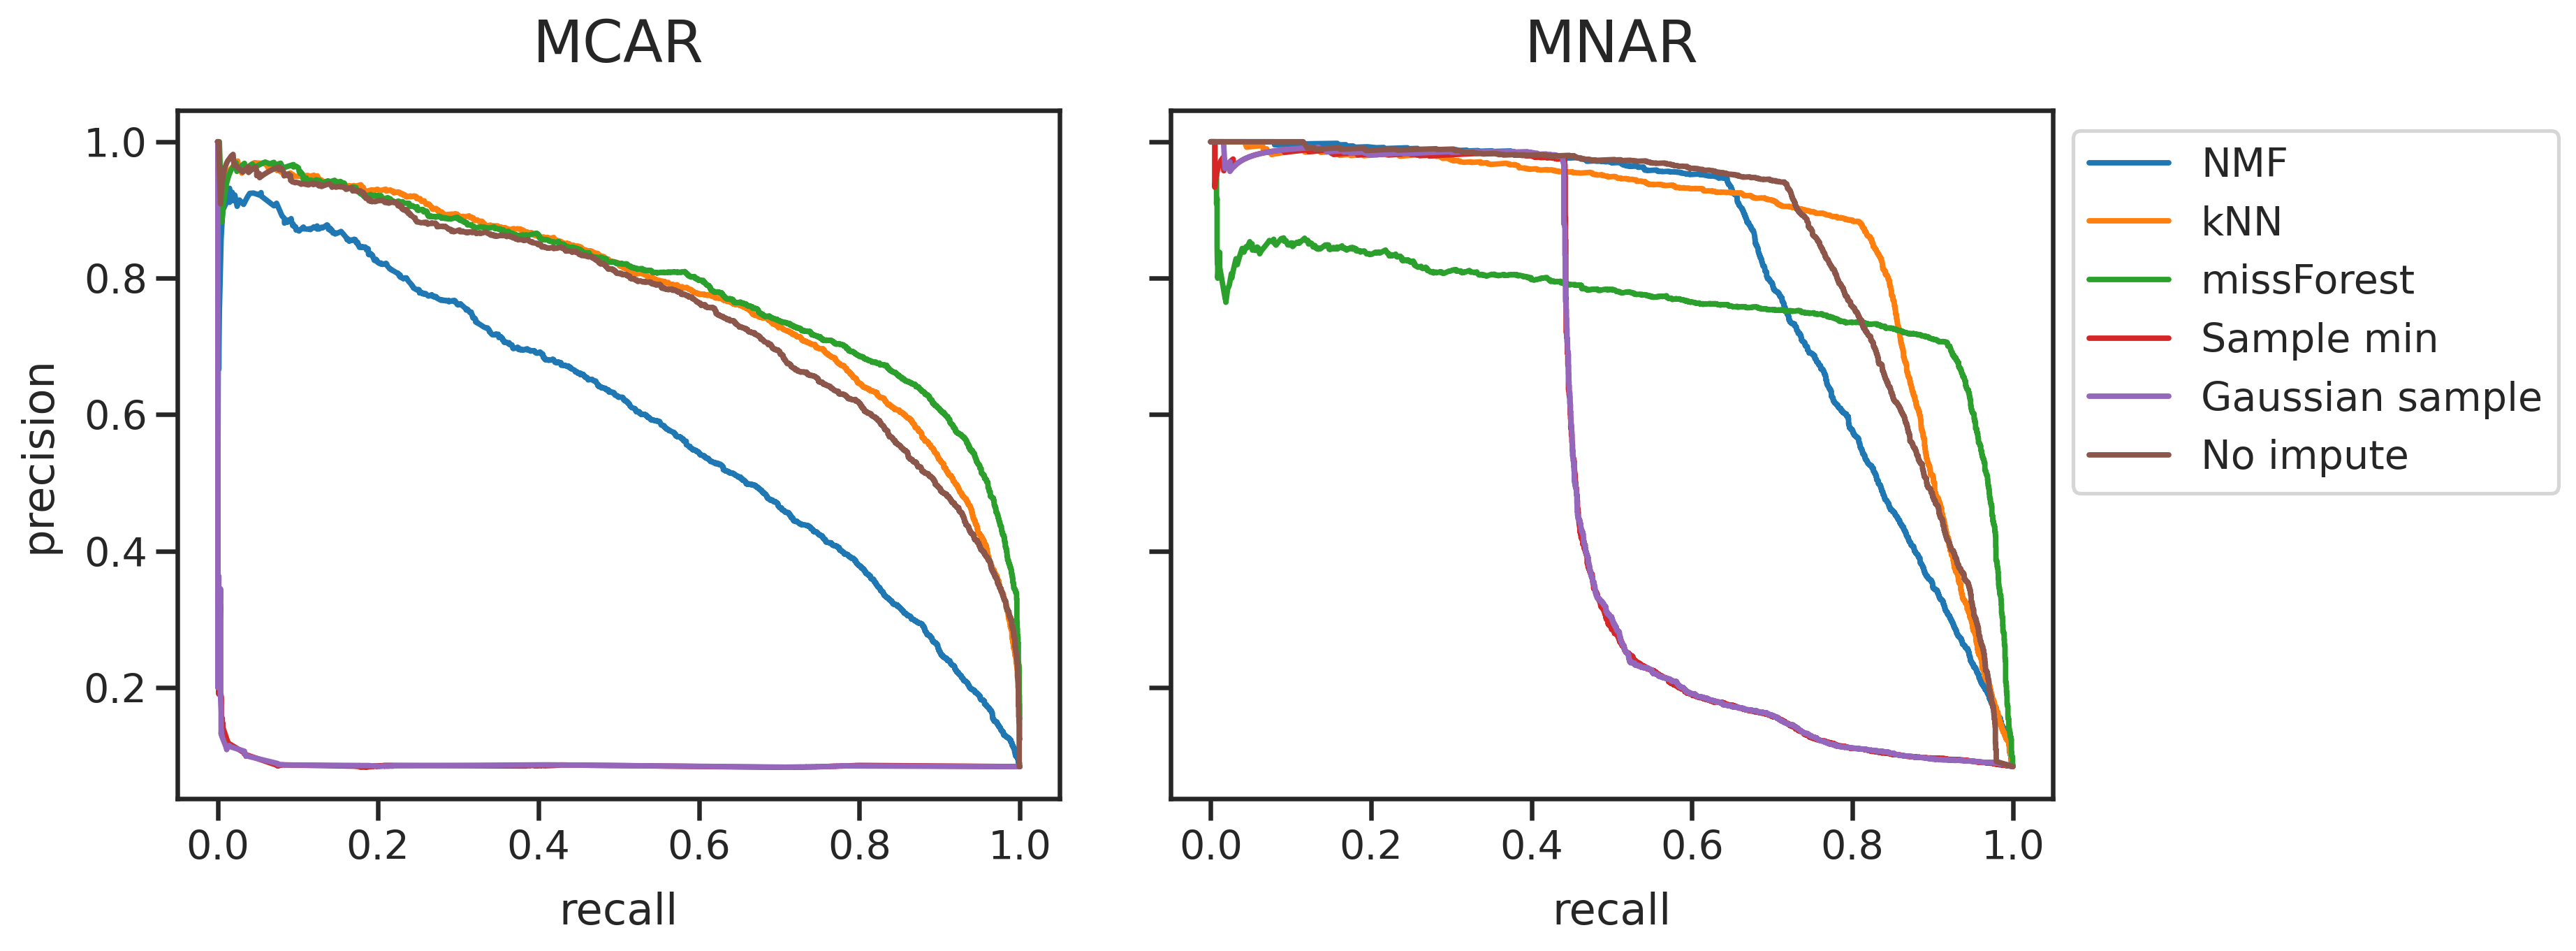
\includegraphics[width=1.0\textwidth]{figures/DE-experiment-multipanel0.png}
\caption{{\bf Evaluating the ability of various MS/MS imputation methods to reconstruct differentially expressed peptides.} Data obtained from PXD034525, a DIA study of Alzheimer's disease. Differentially expressed peptides were identified between samples annotated as (i) autosomal dominant dementia and (ii) high cognitive function, low Alzheimer's disease neuropathologic change \cite{smtg-maccoss}. \textit{Abbreviations:} MCAR: missing completely at random, MNAR: missing not at random. \textit{MCAR AUCs:} NMF: 0.59, kNN: 0.78, \textit{missForest}: 0.8, Sample min: 0.09, Gaussian sample: 0.09, no impute: 0.76. \textit{MNAR AUCs:} NMF: 0.82, kNN: 0.87, \textit{missForest}: 0.77, Sample min: 0.53, Gaussian sample: 0.53, no impute: 0.86.}
\label{fig:PR-curves}
\end{figure}

\begin{figure}
\centering
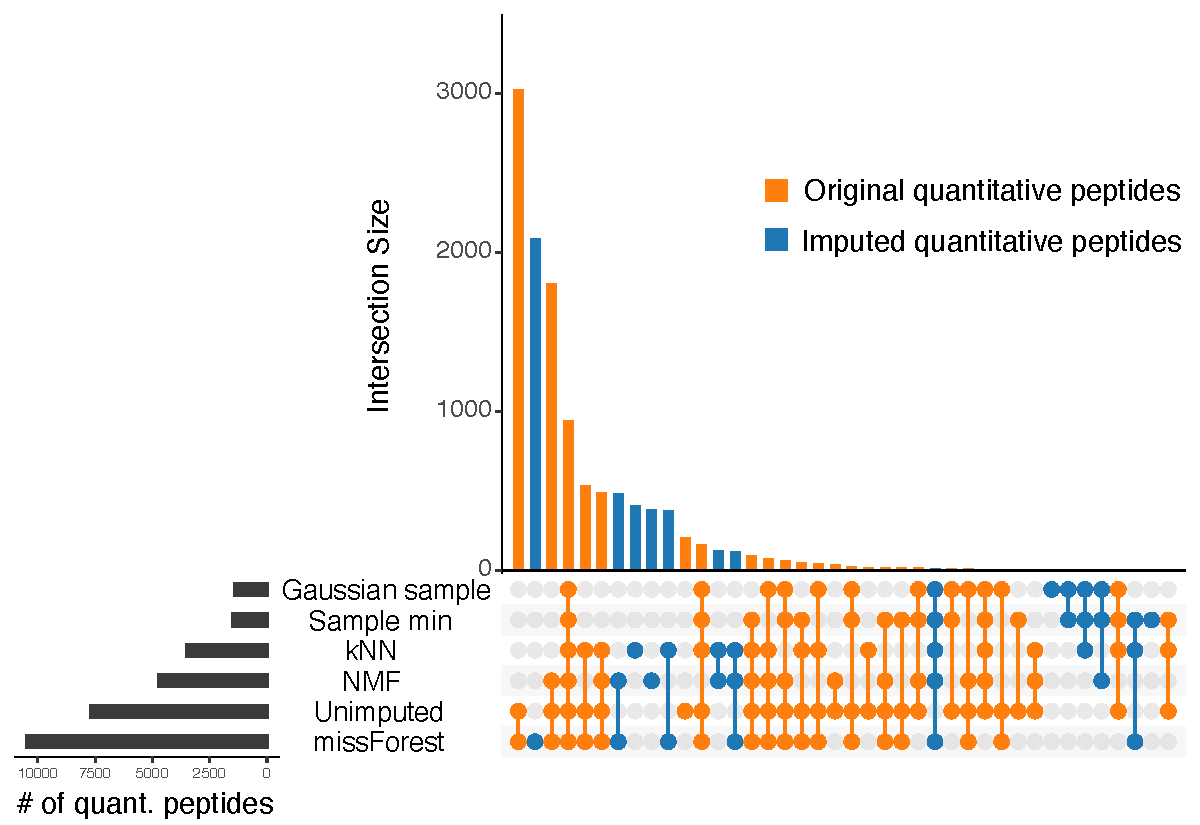
\includegraphics[width=0.9\textwidth]{figures/upset-plot-tab10.pdf}
\caption{{\bf Imputation increases the number of quantitative peptides in a tandem mass spectrometry experiment.} Data obtained from PXD014815 \cite{matrix-matched-calib}. Intersections between unimputed quantitative peptides and post-imputation quantitative peptides are shown in orange. Blue indicates peptides that only become quantitative after imputation.}
\label{fig:rescue-experiment}
\end{figure}

\begin{figure}
\centering
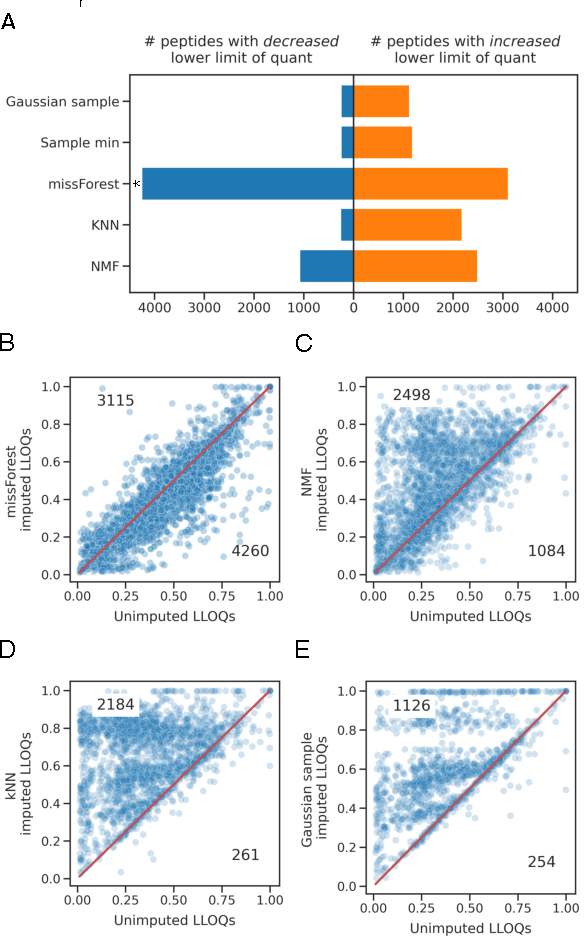
\includegraphics[width=0.65\textwidth]{figures/LLOQ-figure-multipanel-export3.pdf}
\caption{{\bf Imputation changes the lower limit of quantification (LLOQ) for a portion of the peptides in a tandem mass spectrometry experiment.} Data obtained from PXD014815 \cite{matrix-matched-calib}. In (A) the asterisk indicates a one-sided binomial Benjimani-Hochberg corrected p-value $<$0.01. In (B-E) the LLOQs of unimputed peptides are plotted against the LLOQs for the same peptides post-imputation. Only peptides whose LLOQs change post imputation are included.}
\label{fig:lloq}
\end{figure}

\begin{figure}
\centering
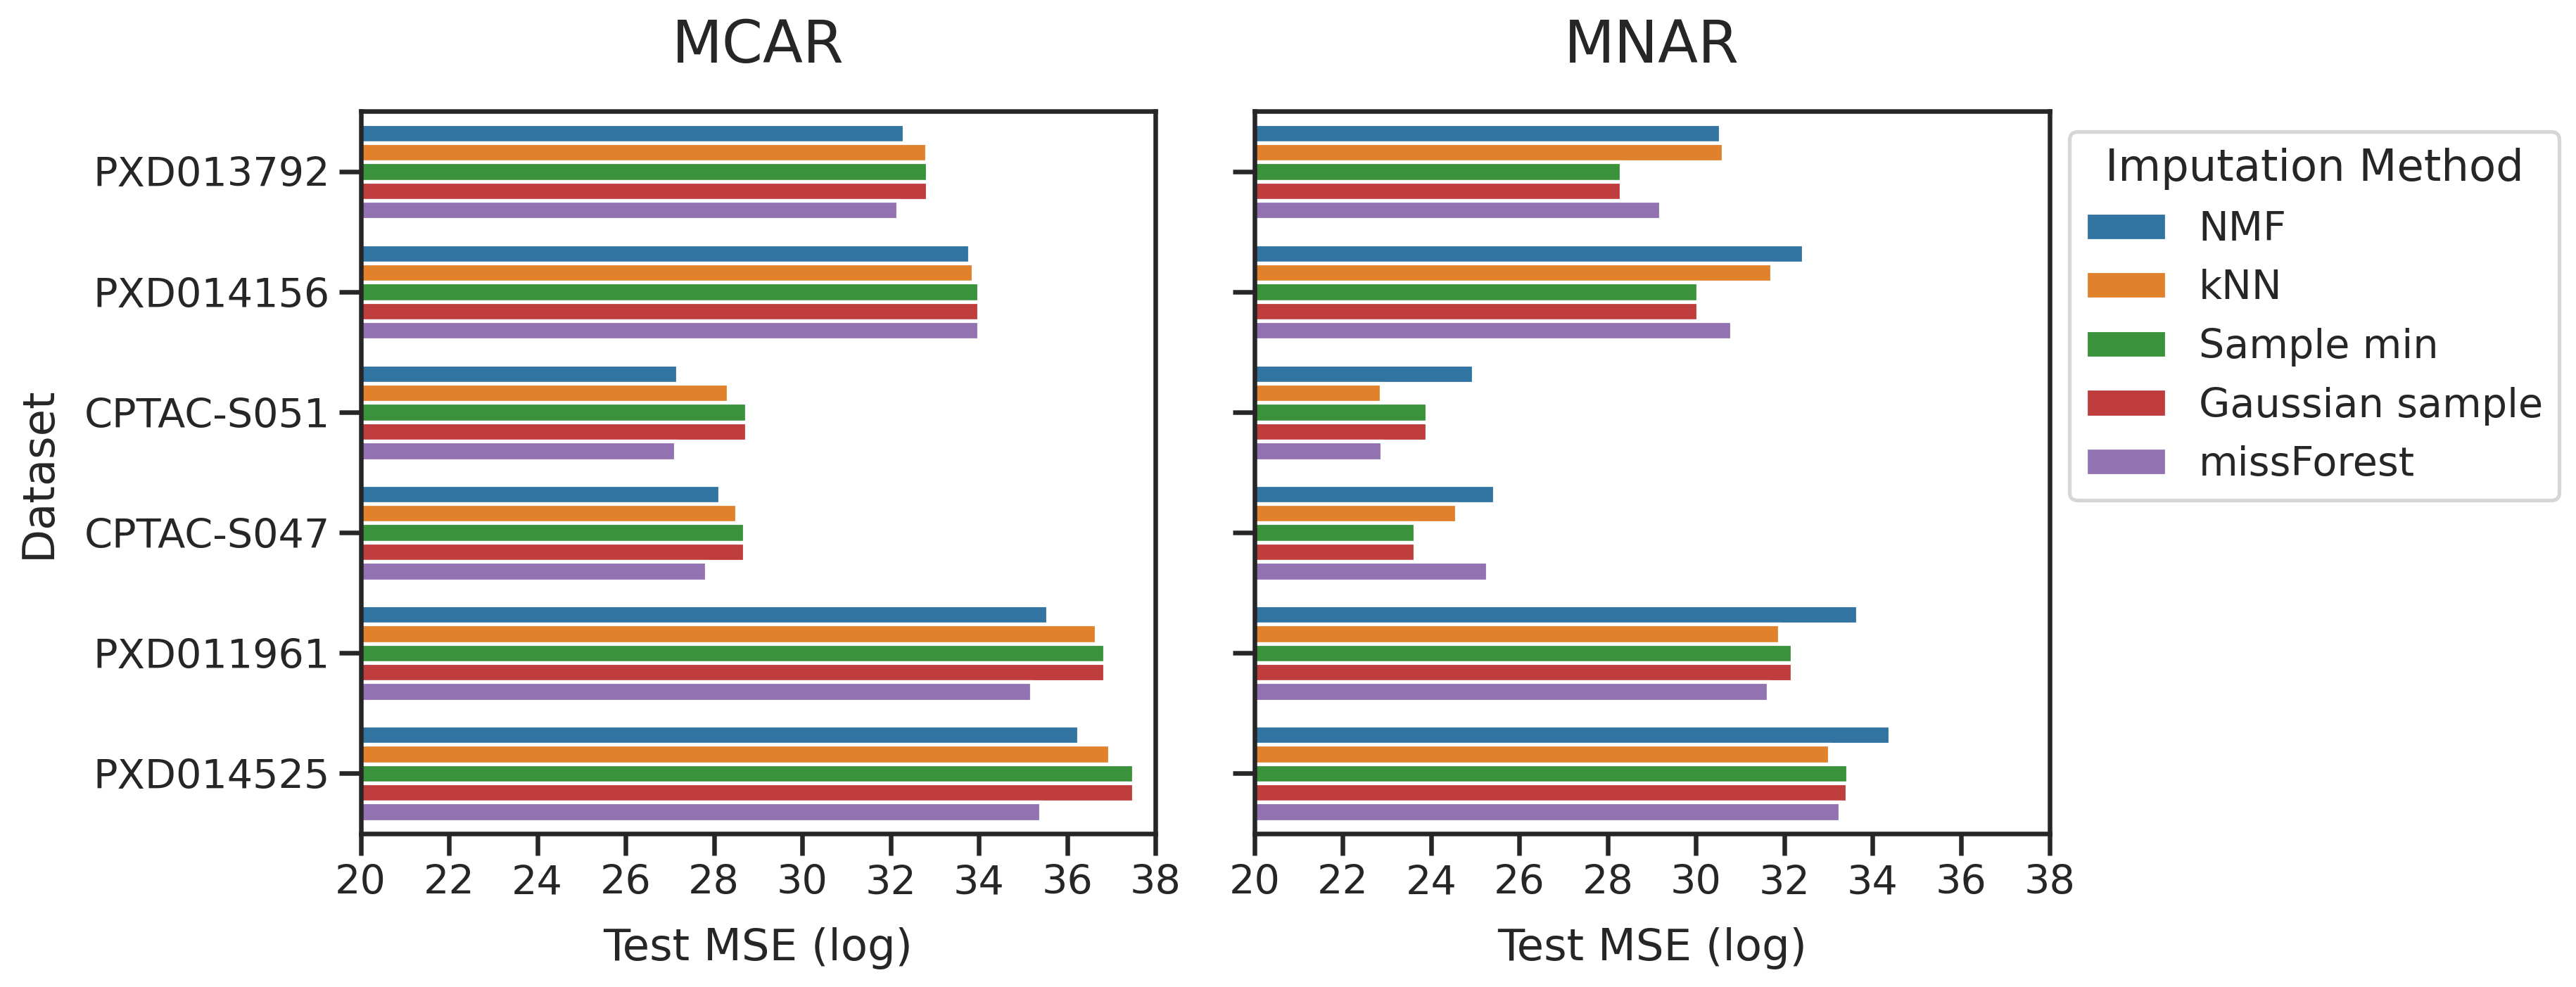
\includegraphics[width=0.95\textwidth]{figures/traditional-barplots-plus-TMT.png}
\caption{{\bf Evaluating MS/MS imputation methods with traditional criteria.} 
Test set MSE after imputation with five methods is shown for six public tandem mass spectrometry datasets. \textit{Abbreviations:} MSE: mean squared error, MCAR: missing completely at random, MNAR: missing not at random.}
\label{fig:traditional-eval}
\end{figure}

\begin{figure}
\centering
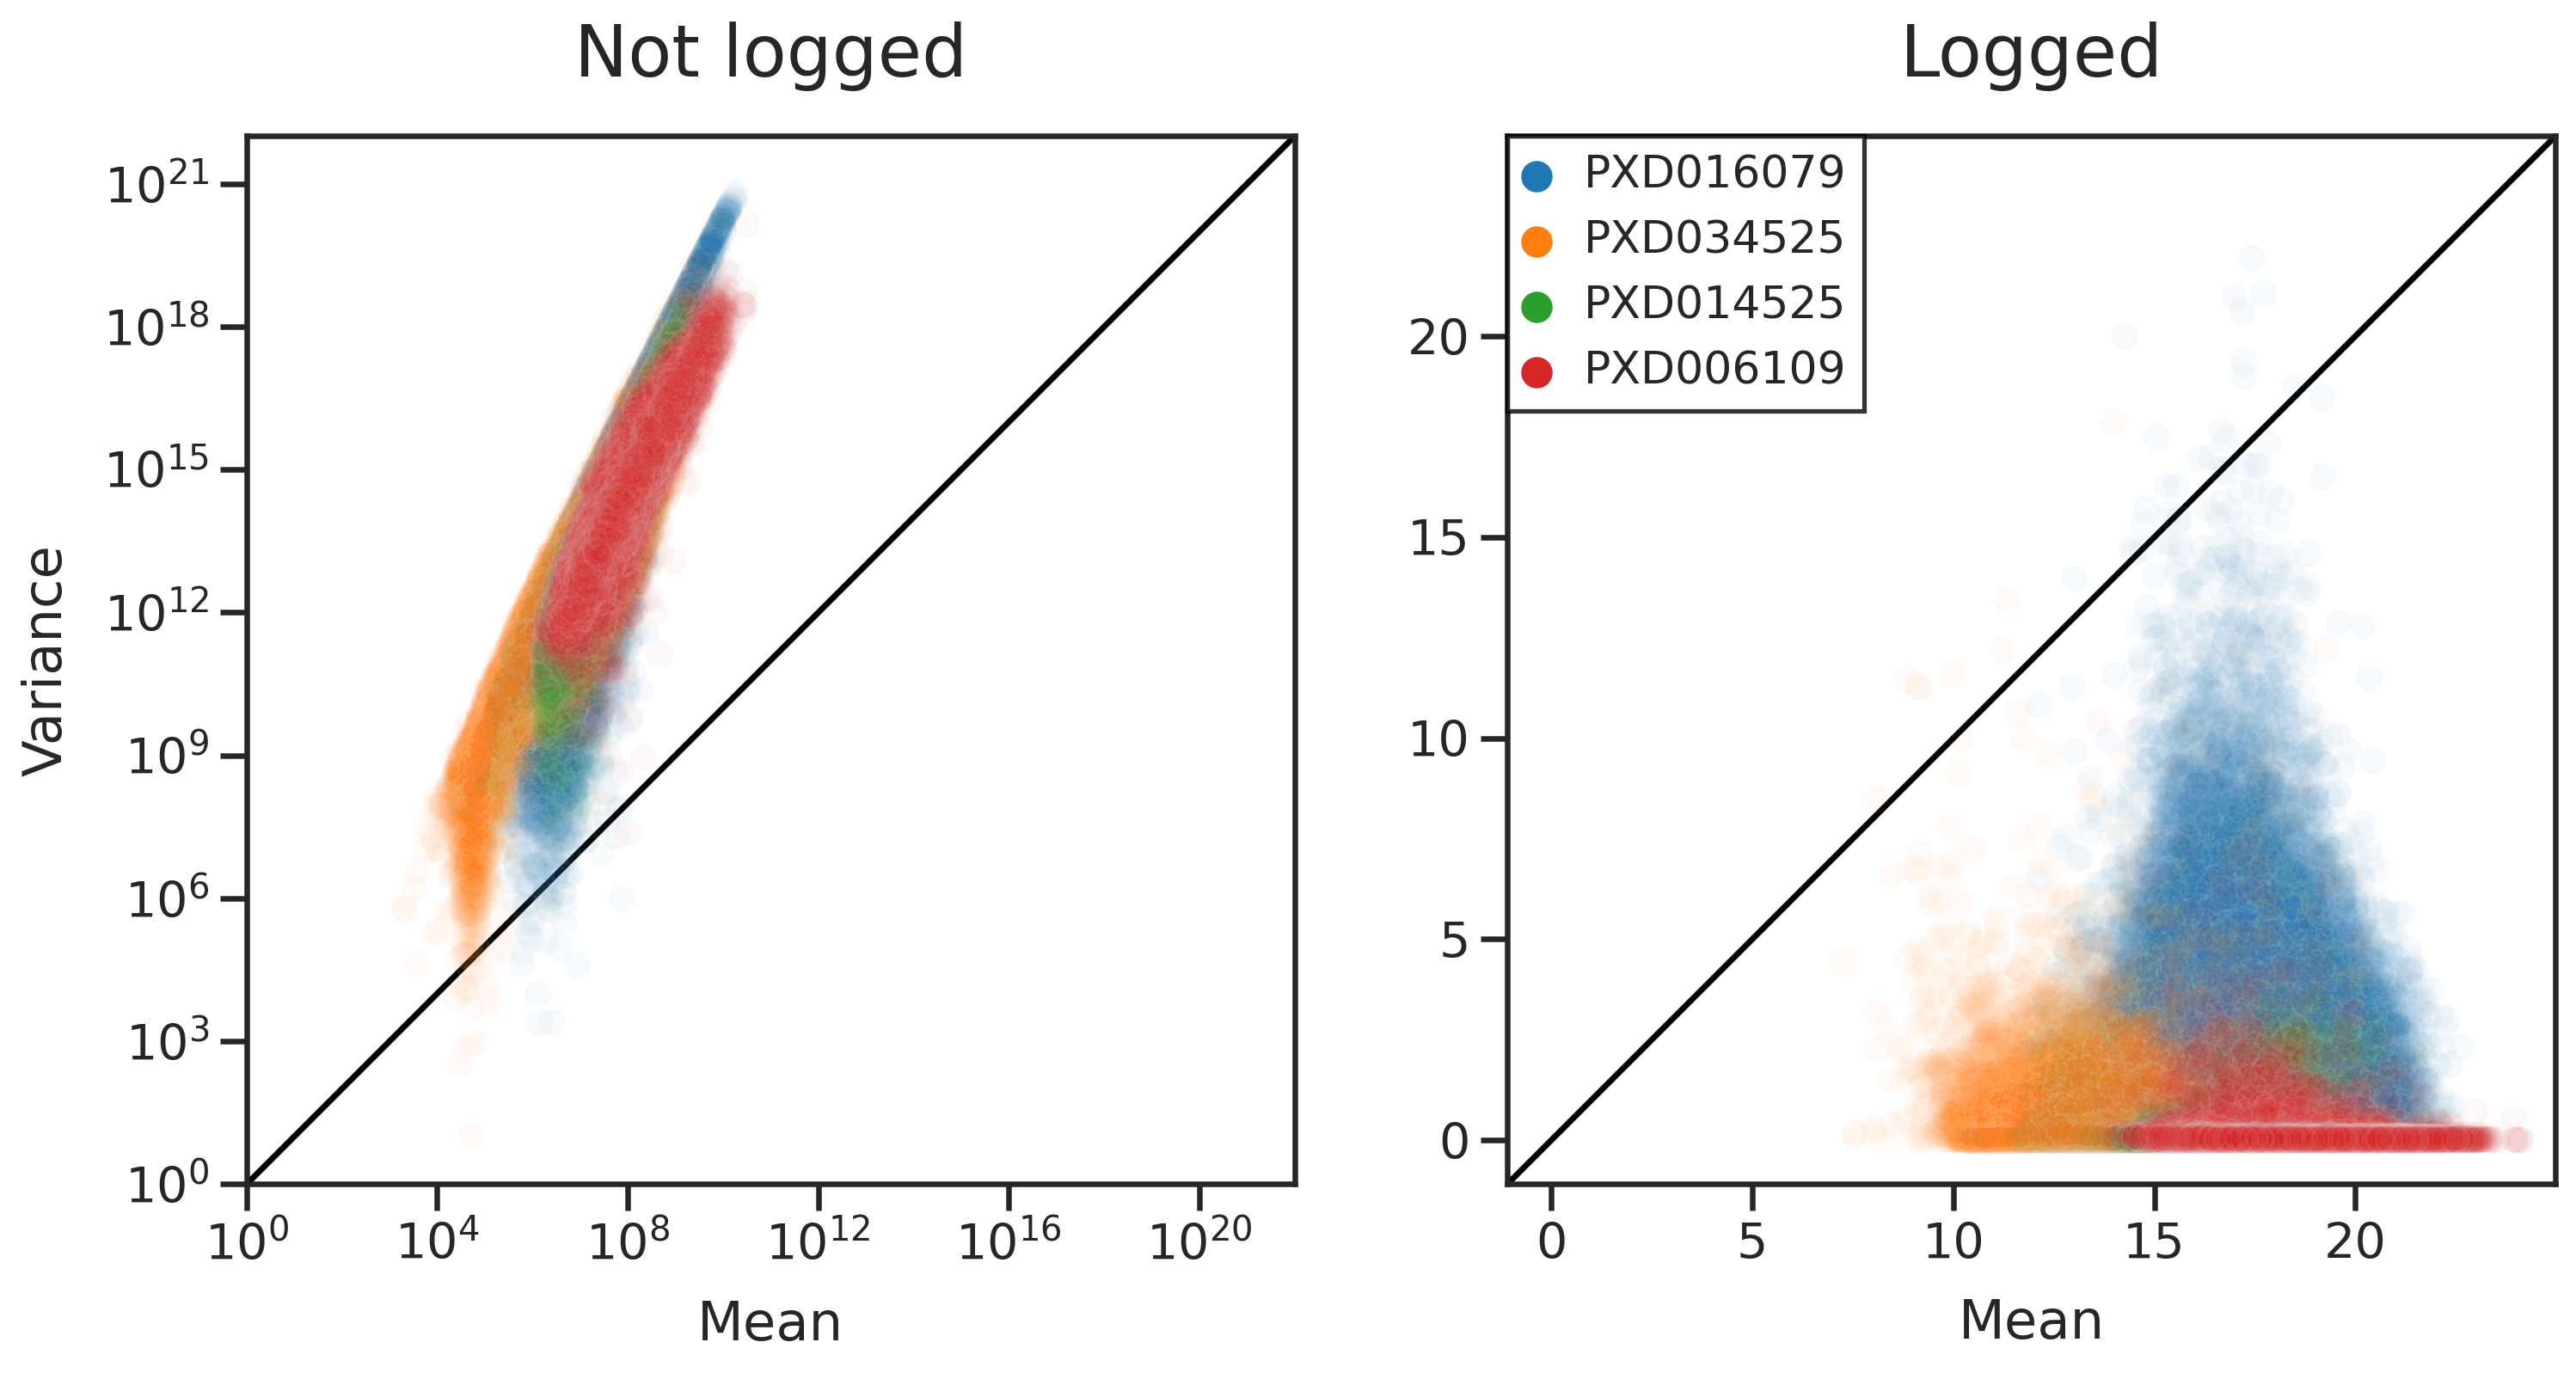
\includegraphics[width=0.8\textwidth]{figures/mean-x-var-figure-v3.png}
\caption{{\bf Quantitative MS/MS data are overdispersed relative to the Poisson distribution.} Means and variances were calculated across technical replicates for four public MS/MS datasets. Peptide level quantifications are shown. The color scheme is the same in both panels. In the right panel, the peptide quantifications were log transformed.}
\label{fig:mean-x-var}
\end{figure}

\begin{figure}
\centering
%\includegraphics[width=0.45\textwidth]{}
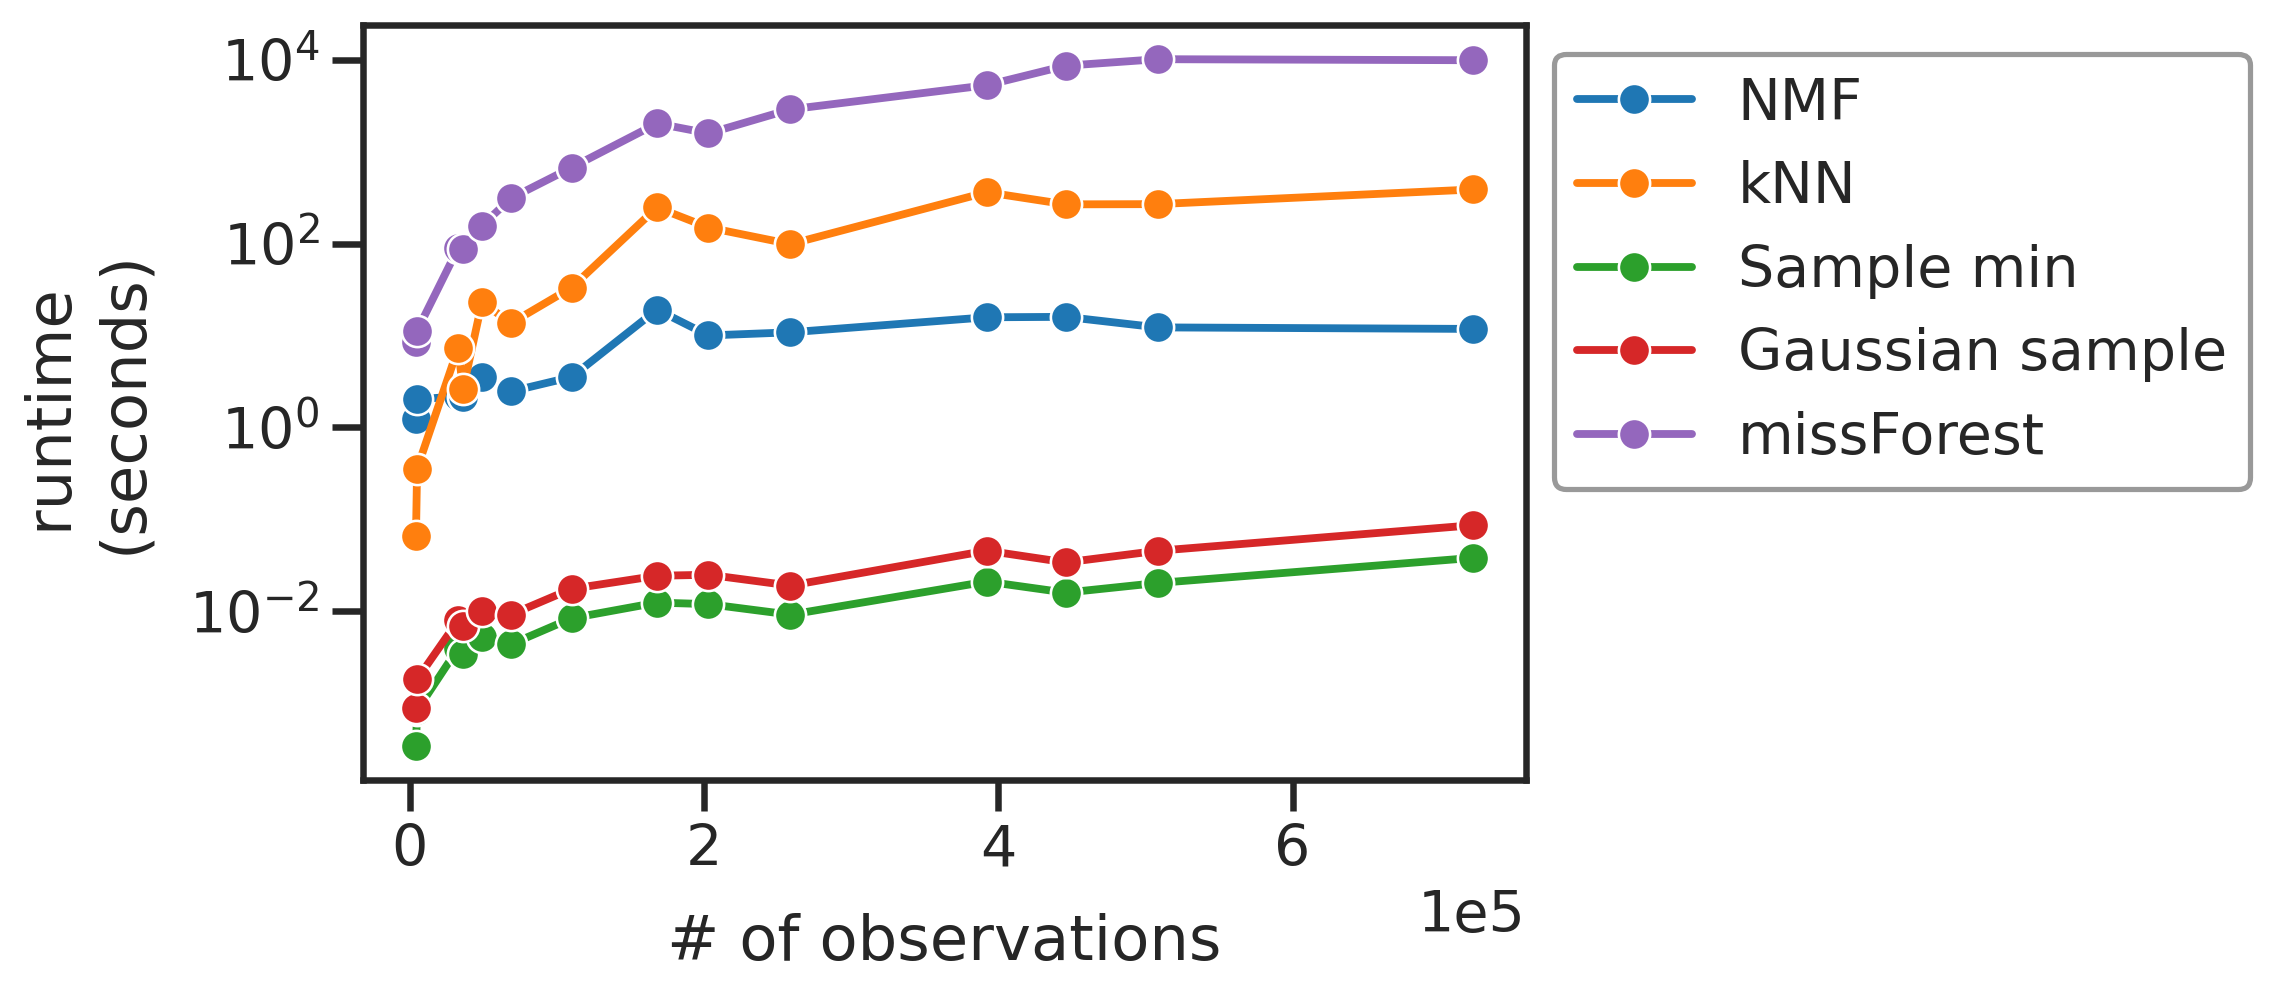
\includegraphics[width=0.8\textwidth]{figures/runtimes-plotted-lineplot-cp.png}
\caption{{\bf Runtime comparison of various MS/MS imputation methods.} Each point represents a public MS/MS dataset. Datasets are ordered by the number of non-missing observations in their training sets after a standard 80\%/20\% train/test partition. Experiment was performed on a dual CPU Intel Xeon E5-2620 machine with 32Gb RAM. 10 cores were provided for NMF, the rest were run on a single core.}
\label{fig:runtime}
\end{figure}

% \begin{figure}
% \centering
% %\includegraphics[width=0.45\textwidth]{}
% %\includegraphics[width=0.4\textwidth]{}
% \caption{{\bf Could we show that imputation improves reproducibility?} Between replicate runs within the same experiment, or perhaps the same samples run on different instruments.}
% \label{fig:reproduce}
% \end{figure}

\section{Discussion}
In spite of the abundance of methods for imputation of quantitative proteomics data, in practice only a small handful of methods are actually used by proteomics researchers. This may be in part due to the fact that many imputation methods are archaic R packages originally intended for microarray imputation. The Perseus strategy of randomly sampling from a Gaussian distribution centered about the lowest observed quantitation value is quite popular, in spite of the fact that multiple studies have demonstrated it ineffectiveness \cite{lazar, Bramer:review, Webb-Robertson:review}. But Perseus is easy to use and is integrated within a commonly used data processing tool, which may explain its popularity. Clearly there is a need for imputation methods that are as easy to use as Perseus but are far more accurate. Perhaps in the future such methods may be integrated into commonly employed proteomics processing workflows and tools. 

We demonstrate that peptide quantifications do not meet certain criteria of the Poisson and Gaussian distributions. This is relevant in the fact that certain imputation methods make implicit distributional assumptions. Any parametric method probably makes the Gaussian assumption. Such parametric methods are thus unlikely to work very well, as they do not properly account for the distribution of quantifications. But it is probably worth pointing out that non-parametric imputation methods (i.e. \textit{missForest} and kNN) are still fine. Also, to our knowledge, it has never been reported that peptide quantifications are overdispersed relative to the Poisson assumption. 

We posit that the proteomics community can borrow knowledge from the single-cell transcriptomics community, which has been modeling counts data with the negative binomial distribution for years.  We specuate that proteomics imputation methods that explicitly model quantitations with the negative binomial distribution may work very well. 

We argue that commonly employed machine learning-style evaluation metrics are less relevant to evaluating the performance of imputation methods than certain proteomic specific criteria. We call for future benchmarking studies to focus mainly on proteomic criteria, as we have done here. 

We find that a high quality imputation method can increase the accuracy of DE peptide detection, increase the number of quantitative peptides and decrease the LLOQ for peptides in a mass spectrometry-based proteomics experiment. These last two conclusions mean that imputation allows for additional peptides to be included in downstream analysis that otherwise would be thrown out. This will increase statistical power and potentially the reproducibility of a proteomics experiment. We argue that imputation should be thought of an analytical procedure that can improve the quality of data generated by a mass spectrometry experiment. 

In light of our proteomics specific criteria we find that \textit{missForest} is generally the best performing imputation method. We speculate that this is because it is non-parametric and thus does not make problematic distributional assumptions. It also is capable of capturing non-linear relationships between input and output variables. 

Modern instruments and experimental protocols enable us to quantify peptides form ever-smaller sample volumes. As input volumes decrease, the missingness problem will only increase. Thus, high quality imputation methods will be essential to meet the demands of single-cell proteomics. 

%\bibliographystyle{plain}
\bibliographystyle{unsrt}
\bibliography{references.bib} 

\end{document}
